\section{Large model}
The memory capacity of the \graicore{} is limited to \SI{36}{MiB}.
Large models have high memory requirements, exceeding its memory capacity, even after applying model optimizations.
The inability to deploy such large models is a consequence of this limitation

We employ splitting of a large model into groups of layers to allow for a large model to be partitioned in parts.
Each part is expected to fit on the \graicore{} and whenever the large model is invoked for execution, each part configured and processed by the \graicore{} sequentially.

When targeting minimal inference latency, we acknowledge that an optimal partitioning strategy for an arbitrary large model is a complex problem to solve.
Therefore, we start with presenting the problem formally.
% In \cref{ch:8}, we present a comprehensive formal description of the problem.

\subsection{Large model partitioning}
We formulate the problem of model partitioning as a multi-objective optimization, aiming to minimize the total inference time while adhering to memory constraints.

With the following given:
\begin{itemize}
    \item A large model with $N$ layers represented as a set $L = \left\{ \, l_1, l_2, \ldots, l_N \, \right\}$.
    \item The \graicore{} with a maximum memory capacity of $M$.
    \item A compiler that can be configured with parameters $\pi_i$ for each partition $p_i$.
    % \item Target total inference latency $T$.
\end{itemize}
We determine an optimal partitioning strategy that divides the model into $K$ consecutive sets of layers ($P = \{p_1, p_2 \ldots, p_K\}$), where each $p_i \subseteq L$, and find the optimal compiler parameters $\pi_i$ for each partition.
This partitioning and parameter selection must minimize the total inference latency, when executing the partitioned model on the \graicore{}, while satisfying the following constraints:

\begin{description}
    % \item[Latency:] 
    % The total inference time consists of the processing time and configuration time of every partition in $P$.
    % The total inference time must not exceed $T$.
    % The value for $T$ is variable and depends on the specific model in question and the requirements from the end-user.
    % \begin{equation}
    %     \lattotal(p_i, \pi_i) = \sum_{i=1}^{K} \left( \latconf(p_i, \pi_i) + \latproc(p_i, \pi_i) \right) \leq T
    % \end{equation}
    \item[Containability:]
    The data size of the partition mapped with some compiler parameters must not exceed the \graicore{}'s total memory capacity $M$.
        The data size of a mapped partition is influenced by the layers contained in the partition and the used compiler parameters ($\writeamount(p_i, \pi_i)$).
    \begin{equation}
        \forall i \in \{i \in \mathbb{N} \mid 1 \leq i \leq K\}, \; \writeamount(p_i, \pi_i) \leq M
    \end{equation}
    \item[Mappability:]
    The partition in combination with some compiler parameters must be mappable with the compiler.
    \begin{equation}
        \forall i \in \{i \in \mathbb{N} \mid 1 \leq i \leq K\}, \; \mappable(p_i, \pi_i)
    \end{equation}
    \item[Exclusiveness:]
    To ensure that the partitioned model maintains the accuracy of the original large model, every layer must belong to exactly one partition.
    \begin{equation}
        \bigcap_{p \in P} p = \emptyset \wedge \bigcup_{p \in P}p = L
    \end{equation}
    \item[Consecutiveness:]
    Each partition is a consecutive subset of layers.
    \begin{equation}
        \forall p \in P, \; p \subseteq \{l_i \in L \mid \alpha \leq i \leq \beta\} \; \text{for} \;  \alpha, \beta, i \in \mathbb{N} \wedge 1 \leq \alpha \leq \beta
    \end{equation}
    % \item[Sequentiality:]
    % to ensure the execution of the partitions happens in a strict sequential manner, we define a relation $\triangleright$ on the set $P$ such that $p_i \triangleright p_j$ if and only if $p_i$ must be executed before $p_j$.
    % This relation adheres to the following axiom:
    % \begin{equation}
    %     \forall i \in \{i \in \mathbb{N} \mid 1 \leq i < K \}, \; p_i \triangleright p_{i+1}
    % \end{equation}
    % This axiom describes that partitions are strictly executed in order of their index. It also implies that:
    % \begin{itemize}
    %     \item No skipping is possible. A partition cannot be executed before another partition that is more than one step ahead. For example, $p_1 \triangleright p_3$.
    %     \item Execution of the same partition in sequence is not allowed (e.g., $p_1 \triangleright p_1$).
    % \end{itemize}
\end{description}

The objective is to minimize the total inference latency with the partitioned model on the \graicore{}.
The total inference latency consists of the processing time and configuration time of every partition in $P$.

\begin{align*}
    \textrm{minimize} & \quad \sum_{i=1}^{K} \left( \latconf(p_i, \pi_i) + \latproc(p_i, \pi_i) \right) \\
    \textrm{subject to} & \quad \textrm{(the contraints above)}
\end{align*}

\begin{eqexpl}[30mm]
    \item{$\latconf(p_i, \pi_i)$} configuration time for model part $p_i$ with compiler parameters $\pi_i$
    \item{$\latproc(p_i, \pi_i)$} processing time for model part $p_i$ with compiler parameters $\pi_i$
\end{eqexpl}

\subsubsection{Scope and limitations}
The primary focus is on layer-wise partitioning, where the model is divided into consecutive sets of layers.
We do not explore alternative techniques such as tensor partitioning or pipeline execution (where configuration and processing are executed in parallel), which might offer advantages in certain scenarios.
This approach is chosen for its relative simplicity and its ability to preserve the inherent structure of the original model, ensuring functional correctness and minimizing the potential of accuracy degradation.

Additionally, we focus on static partitioning, where the partitioning scheme is determined before runtime.
Also, we treat the compiler for the \graicore{} as a black box, focusing on exploring the effects of adjusting available compiler parameters on inference latency.

We acknowledge that our model of the \graicore{} simplifies certain aspects of the hardware.
For instance, we represent the \graicore{}'s SRAM memory as one large memory, while in reality, it is comprised of $144$ smaller SRAMs.

Lastly, our focus is on partitioning strategies where each partition is executed only once in a sequential manner.
While we acknowledge the potential benefits like data reuse and reduced configuration overhead of executing the same partition multiple times in sequence (e.g., for models with recurrent connections), exploring such strategies is beyond the scope of this work.

%%%
% In this section, we analyze the execution of such large models.
% As a large model can be of any size that can be split with in an arbitrary amount of parts, and with each part having its own processing latency, no bandwidth requirement is suitable for all large models.

\subsection{Bandwidth analysis}
To target a specific input frame rate with a large model, we require information for the following components:
\begin{itemize}
    \item Number of model parts
    \item Configuration time for each model part, which depends on:
    \begin{itemize}
        \item Write bandwidth
        \item Amount of data to be written for each model part
    \end{itemize}
    \item Processing time for each model part
\end{itemize}

We estimate the maximum reachable input frame rate ($f$) as follows:
\begin{align*} 
    \lattotal &= \sum_{p \in P}^{}{\latconf(p) + \latproc(p)} \\
    f &= \lattotal^{-1}
\end{align*}

\begin{eqexpl}[15mm]
    \item{$\lattotal$} total latency
    \item{$P$} set of model parts
    \item{$\latconf(p)$} configuration time for model part $p$
    \item{$\latproc(p)$} processing time for model part $p$
\end{eqexpl}

For example, assume we have a large model partitioned into four parts with each part requiring \SI{20}{MiB} to be written and has \SI{5}{ms} of processing latency.
The total latency is then only dependent on the available bandwidth, as it influences the configuration time:
\begin{equation*}
    f = \left[ \left( \frac{\SI{20}{MiB}}{\textrm{BW}} + \SI{5}{ms} \right) \times 4 \right]^{-1}
\end{equation*}

\begin{eqexpl}[15mm]
    \item{$\textrm{BW}$} available bandwidth
\end{eqexpl}

\begin{figure}
    \centering
        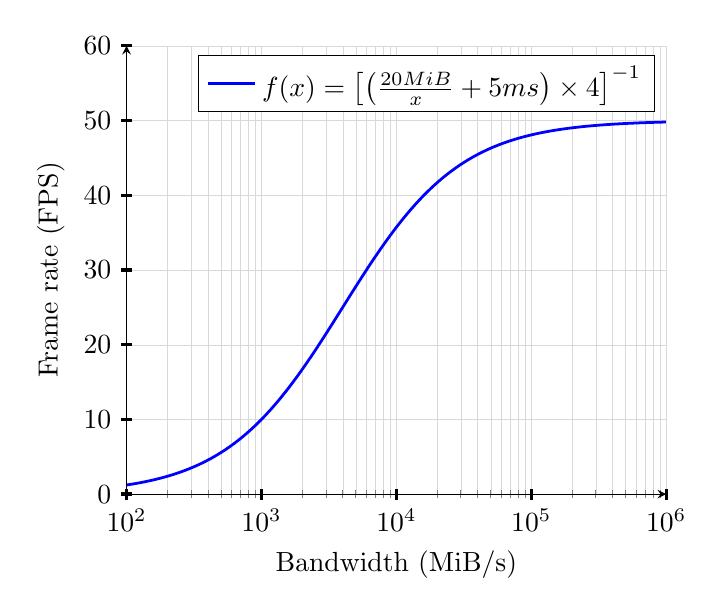
\begin{tikzpicture}
    \begin{semilogxaxis}[
        axis lines = left,
        xlabel = {Bandwidth (MiB/s)},
        ylabel = {Frame rate (FPS)},
        ymin = 0, ymax = 60,
        xmin = 100, xmax = 1000000,
        ytick distance=10,
        grid=both,
        grid style={line width=.1pt, draw=gray!30},
        every major tick/.append style={very thick, major tick length=4pt, black},
    ]
    
    \addplot [
        domain=1:1000000, 
        samples=1000, 
        color=blue,
        line width=1pt
    ]
    {1/((20/x + 0.005)*4)};
    
    \addlegendentry{$f(x) = \left[ \left( \frac{\SI{20}{MiB}}{x} + \SI{5}{ms} \right) \times 4 \right]^{-1}$}
    \end{semilogxaxis}
    \end{tikzpicture}

    \caption{Reachable frame rates with varying bandwidths for an example large model}
    \label{fig:large_model_bandwidth_analysis_example}
\end{figure}

\Cref{fig:large_model_bandwidth_analysis_example} shows that there is an horizontal asymptote at \SI{50}{FPS}\footnote{ $\lim_{x \to \infty} \left[ \left( \frac{\SI{20}{MiB}}{x} + \SI{5}{ms} \right) \times 4 \right]^{-1} = \SI{50}{Hz}$}.
Due to this, it is not possible to target an input frame rate of \SI{60}{FPS} for this model.
Even with an infinite write bandwidth, we can never reach \SI{60}{FPS}.
This limitation is due to the fixed processing latency of the four model parts (\SI{20}{ms}).
An input frame rate of \SI{30}{FPS} is possible and requires a write bandwidth of at least \SI{6}{GiB/s}.

With the bandwidth of the baseline \confignoc{} (\SI{763}{MiB/s}), we can target up to \SI{8}{FPS}\footnote{$\left[ \left( \frac{\SI{20}{MiB}}{\SI{763}{MiB/s}} + \SI{5}{ms} \right) \times 4 \right]^{-1} \approx \SI{8}{Hz}$}.

\subsection{Execution of the ResNet-101 model}
We will be looking at the execution of a large model named ResNet-101 on the \graicore{}.
The ResNet-101 model is a deep neural network commonly used for image recognition \autocite{heDeepResidualLearning2015}.
We will be using the ResNet-101 model from the \textit{Keras} library \cite{chollet2015keras} pretrained on the ImageNet database \cite{russakovskyImageNetLargeScale2014}.
The ResNet-101 model has around 44.5 million parameters in total.
% An important feature of the ResNet architecture is the use of skip connections \cref{TODO}.

Due to the size (amount of parameters) of the ResNet-101 model, it is not possible to load the model on the \graicore{} at once.
This is still the case when the parameters are quantized using a lower-resolution data type 8-bit integers or floats.
% Other solutions, such as model compression techniques, exist to decrease the size of the model.
% However, as explained earlier, this has its disadvantages such as decreased inference accuracy.
Other model compression techniques can be applied to offer a way to reduce model size.
However, this advantage often comes with a trade-off, leading to decreased inference accuracy as previously discussed.

% TODO: refer to the DEFER paper
% layer-wise partitiong figure
% \begin{figure}[hbtp]
%     \centering    
%     \includegraphics[width=3cm]{example-image-a}
%     \caption{TODO: partitioning of a model diagram}
% \end{figure}

To allow the model to fit on the \graicore{} we will be looking at partitioning the model into smaller parts.
A model part should be small enough to completely fit on the \graicore{}
By sequentially loading and processing each of the model parts, the full functionality of the original (large) model can be emulated.
The output data of each model part must be buffered outside the local memories, and will be used as input for the subsequent model part.
The amount of data to be buffered is dependent on the output shape of the final layer of a part.
% TODO where are they stored?

\begin{figure}[hbtp]
    \centering
    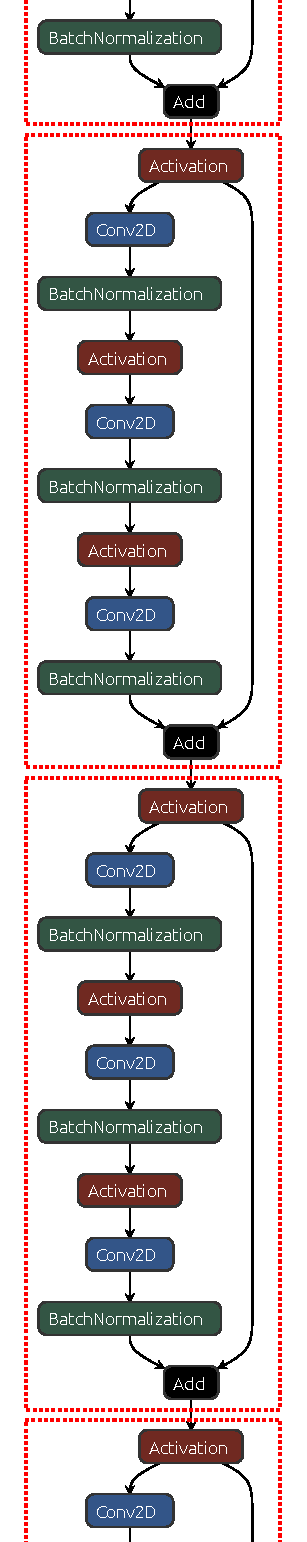
\includegraphics[angle=90, width=\linewidth]{assets/resnet101_residual_blocks.pdf}
    \caption{
    Snippet of a visualization of the ResNet-101 network.
    The red rectangles represent the residual blocks.
    }
    \label{fig:resnet101_residual_blocks}
\end{figure}

The ResNet architecture introduces so-called residual blocks (see \cref{fig:resnet101_residual_blocks}).
A residual block contains a collection of layers with a special type of connection from the beginning of the block until the end of the block.
This connection is also called a skip connection.
Due to these skip connections, it is not straightforward to split the ResNet-101 model at any location.
Splitting the model between two layers where also a skip connection resides, will introduce a few difficulties.
Firstly, multiple outputs are required to be buffered.
That is, the output data of the layer just before the split point and the output data of the skip connection.
Secondly, the two outputs need to be propagated to their respective destination layers.
These two outputs can have the same or different destination layer.
If they have different destinations, the output of the skip connection needs to be buffered until the network reaches a later stage.

In the context of the \graicore{}, this adds extra complexities to the system.
Not only does this increase the instantaneous total memory usage, but also increases the energy usage.
More energy is consumed due to the increased data to be buffered.
This is especially evident due to the need to buffer the data on some external memory.
In addition to this buffering problem, this also requires software support.
The current system only allows for a single input to the model. 

Due to these complexities, we only consider partitioning the network at locations where no skip connections appear.
Naturally, the main drawback of this is the reduced number of locations where partitioning can occur.

\begin{figure}[hbtp]
    \centering
    \subcaptionbox{MACs per residual block \label{fig:resnet101_macs}}[\textwidth]{
        \pgfplotstableread[col sep=semicolon]{assets/resnet101_stats.csv}\datatable
\begin{tikzpicture}
    \begin{axis}[
        width=\textwidth,    % set width
        height=0.3\textwidth, % and height
        ybar,
        enlarge x limits={rel=0.05},
        bar width=8pt,   % they were too wide
        xlabel={Residual block},
        ylabel={MACs},
        xlabel style={yshift=-1em},
        xtick=data,
        xticklabel style={rotate=45, font=\scriptsize, anchor=east},
        xticklabels from table={\datatable}{index},
    ]
    \addplot table[x expr=\coordindex, y={macs}]{\datatable};
    \end{axis}
\end{tikzpicture}

    }
    \subcaptionbox{Number of parameters per residual block \label{fig:resnet101_params}}[\textwidth]{
        \pgfplotstableread[col sep=semicolon]{assets/resnet101_stats.csv}\datatable
\begin{tikzpicture}
    \begin{axis}[
        width=\textwidth,    % set width
        height=0.3\textwidth, % and height
        ybar,
        enlarge x limits={rel=0.05},
        bar width=8pt,   % they were too wide
        xlabel={Residual block},
        ylabel={\# Parameters},
        xlabel style={yshift=-1em},
        xtick=data,
        xticklabel style={rotate=45, font=\scriptsize, anchor=east},
        xticklabels from table={\datatable}{index},
    ]
    \addplot table[x expr=\coordindex, y={params}]{\datatable};
    \end{axis}
\end{tikzpicture}
    }
    \caption{
        MACs and the number of parameters per residual block.
        The tuple $(x, y)$ represents the residual block at index $y$ of the stage at index $x$.
        \textit{Head} and \textit{tail} contain the remaining layers at the start and end of the network respectively.
    }
    \label{fig:resnet101_stats}
\end{figure}

The ResNet-101 model contains five so-called stages.
A stage is a collection of consecutive residual blocks.
Only the first stage does not include any residual blocks.
The other stages contain different amounts of residual blocks as shown in \cref{fig:resnet101_stats}.

If we opt to split the network based on computational complexity, we look at the amount of multiply-accumulate (MAC) operations of the layers.
A MAC operation is essentially a multiplication operation followed by an addition operation.
Since we only perform splits between residual blocks, we combine the MACs of each layer in the residual blocks.
In \cref{fig:resnet101_macs}, we observe that the amount of MACs for each residual block is relatively similar.
We see small peaks at the start of each stage.
This is due to an additional convolution layer in the first residual block of a stage.
% A model or model part with more MACs generally is more heavy to run than those with less MACs (lower .
Generally, a model or model part with high number of MACs take longer to process fully.

In \cref{fig:resnet101_params}, we observe that the distribution of the parameters do vary significantly over the residual blocks.
The graph shows that the last few residual blocks carry a significant portion of the total parameters.
Again, we see small peaks at the start of each stage.
Naturally, a model part with a higher number of parameters will require more memory space.
Due to the uneven distribution of the parameters we have less flexibility with partitioning. 

\subsubsection{Splitting}
The ResNet-101 model has a total parameter count of around \SI{44.5}{M}.
Even if the parameters are quantized to an 8-bit datatype, the model will still not fit on the \graicore{} as a whole.
Weights stored on the \graicore{} require one extra bit.
% This extra bit is used as a mask that activates or deactivates the associated weight.
This extra bit is used to indicate whether a weight is removed (i.e., pruned) or not.
However, since we are using the original ResNet-101, no pruning has been applied to the weights.
We can roughly say that the network requires \SI{47.7}{MiB}\footnote{$\frac{\num{44496488} \times 9}{8} \times \frac{1}{2^{20}}$} of memory capacity for the parameters when quantized to 8 bits.
However, this does not include any mandatory header information and buffer space when mapping the network for the \graicore{}. 

We use the compiler to find a valid mapping for the \graicore{}, with focus on low processing latency.
The compiler also outputs files necessary for simulating the networks with a proprietary performance simulator.
This performance simulator is used to estimate the processing latency of each part.
Note that the compiler is a complex piece of software.
Since it accepts many parameters that affects the processing latency, it is difficult to find an optimal mapping. 
% The in-house compiler for the \graicore{} is complex and we will not get into detail.
In a nutshell, the compiler first optimizes the model by converting it to a so-called \textit{GrAI Model}.
Among other things, the optimized model slightly changes the architecture of the network and optionally performs post training quantization \autocite{krishnamoorthiQuantizingDeepConvolutional2018} for the weights.
The amount of MACs and parameters stay roughly the same.
% The compiler can be instructed to optimize for inference latency.
The compiler can be instructed to perform certain optimizations for inference latency.
Afterwards, it will map the layers of the model to the neuron cores.
% One of the optimization is, for example, mapping a single layer to multiple neuron cores to exploit parallelism.

% One example partitioning is done as follows.
The following example illustrates a partitioning scheme.
The splitting points are performed right after the following residual blocks: $(4, 6)$, $(4, 12)$, $(4,21)$ and $(5,1)$.
These splitting points were chosen such that each part contains a chunk of the total parameters with sufficient room to spare for other necessary data.
The ResNet-101 model is therefore partitioned in five parts.
The compiler is able to compile each of the parts, indicating that they are configurable and executable on the \graicore{}.
The processing latency for each of the parts are then estimated using the performance simulator.

An attempt has been made to instruct the compiler to optimize the parts for processing latency.
The compiler parameters have a significant influence on the end results of a model part.
Not only does it influence the size of the mapped model, but it also influences the processing latency.
By instructing the compiler to segment individual layers, we can achieve lower processing latency.
Layer segmentation involves dividing a layer's operations and data across multiple neuron cores, allowing them to process different parts concurrently.
This is particularly beneficial for convolutional layers, where inherent parallelism can be exploited by distributing computations across neuron cores
By keeping the data local to the neuron cores processing it, segmentation minimizes data movement and communication overhead.
However, this increases the total mapped model size as certain weights need to be shared between the neuron cores.
Furthermore, it is also beneficial for the processing latency to involve as many neuron cores as possible for the execution of the model parts.

\begin{table}[hbtp]
\centering
\begin{tabular}{@{}lll@{}}
\toprule
\textbf{Part}  & \textbf{To write (MiB)} & \textbf{Latency (ms)} \\ \midrule
1              & 28.75                   & 7.08                  \\
2              & 20.06                   & 2.65                  \\
3              & 30.44                   & 4.01                  \\
4              & 17.71                   & 2.34                  \\
5              & 15.54                   & 2.04                  \\ \midrule
\textbf{Total} & 112.51                  & 18.12                 \\ \bottomrule
\end{tabular}
\caption{Statistics of the example partitioning of the ResNet-101 model in 5 parts}
\label{tab:resnet101_5parts}
\end{table}

% Note that the compiler can map a layer to multiple neuron cores.
% This requires the weights to be written to all neuron cores that require them.
% This means that the \graicore{} contains duplicate weights.
The compiler also provides us information about how much data must be written to each of the neuron cores.
The total data to write and the processing latency for each part is shown in \cref{tab:resnet101_5parts}.

\begin{figure}[hbtp]
    \centering
        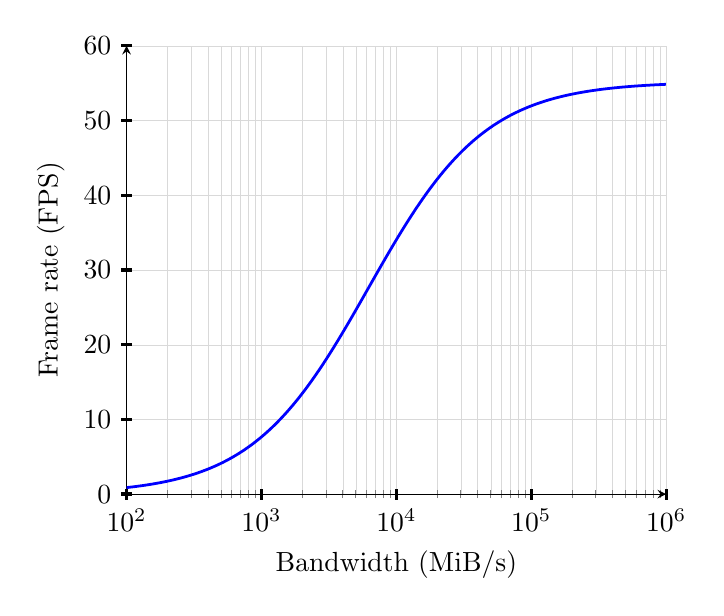
\begin{tikzpicture}
    \begin{semilogxaxis}[
        axis lines = left,
        xlabel = {Bandwidth (MiB/s)},
        ylabel = {Frame rate (FPS)},
        ymin = 0, ymax = 60,
        xmin = 100, xmax = 1000000,
        ytick distance=10,
        grid=both,
        grid style={line width=.1pt, draw=gray!30},
        legend pos={north west},
        every major tick/.append style={very thick, major tick length=4pt, black},
    ]
    
    \addplot [
        domain=1:1000000, 
        samples=1000, 
        color=blue,
        line width=1pt
    ]
    {1/( ((28.75/x) + (7.08/1000)) + ((20.06/x) + (2.65/1000)) + ((30.44/x) + (4.01/1000)) + ((17.71/x) + (2.34/1000)) + ((15.54/x) + (2.04/1000)) )};
    % \addlegendentry{TODO}
    \end{semilogxaxis}
    \end{tikzpicture}

    \caption{Reachable frame rates with varying bandwidths for the example partitioned ResNet-101 model}
    \label{fig:large_model_bandwidth_analysis_example_resnet101}
\end{figure}

The sum of the processing latencies is \SI{18.12}{ms}.
The available time for the configuration of all parts is dependent on the target frame rate.
We observe that it is not possible to target a frame rate of \SI{60}{FPS}.
This is due to the total processing latency exceeding the frame time of \SI{16.67}{ms}. 
For a target frame rate of \SI{30}{FPS}, we have a frame time of \SI{33.33}{ms}.
For the configuration of the parts, we have a total time budget of \SI{15.12}{ms}\footnote{$\SI{33.33}{ms} - \SI{18.12}{ms}$}.
To write all the \SI{112.51}{MiB} to configure each model part, we require a bandwidth of at least \SI{7441}{MiB/s}\footnote{$\frac{\SI{112.51}{MiB}}{\SI{15.12}{ms}}$}.
\Cref{fig:large_model_bandwidth_analysis_example_resnet101} shows the reachable frame rates with different bandwidths.

% The compiler accepts many parameters that can affect the performance (e.g., inference latency or power usage) when the model is running on the \graicore{}.




%%%

% There are many ways to partition a model. 
% Amount of parts (there is a minimum)
% Distribution of parameters
% Distribution of FLOPS/MACs

% We use the in-house compiler to find a valid mapping for the \graicore{}, with focus on low processing latency. The compiler also outputs files necessary for simulating the networks with \graipefruit{}. \graipefruit{} is used to approximate the processing latency of a network.
% Note that the compiler is a complex piece of software. Since it accepts many parameters, it is difficult to find an optimal mapping. 
